\documentclass{article}

\usepackage{fancyhdr}
\usepackage{extramarks}
\usepackage{amsmath}
\usepackage{amsthm}
\usepackage{amsfonts}
\usepackage{tikz}
\usepackage[plain]{algorithm}
\usepackage{algpseudocode}
\usepackage{graphicx}
\usepackage{gensymb}
\usepackage{calc}
\usepackage[framed,numbered,autolinebreaks,useliterate]{mcode}
\usepackage{listings}
\usepackage{empheq}
\usepackage{enumitem}
\usepackage[font=footnotesize]{caption}
\usepackage{subcaption}
\usepackage{lipsum}
\usepackage[export]{adjustbox}

\graphicspath{{./images/}}

\usetikzlibrary{automata,positioning}

%
% Basic Document Settings
%

\topmargin=-0.45in
\evensidemargin=0in
\oddsidemargin=0in
\textwidth=6.5in
\textheight=9.0in
\headsep=0.25in

\linespread{1.1}

\pagestyle{fancy}
\lhead{\hmwkAuthorLastNames}
\chead{\hmwkClass\ \hmwkTitle}
\rhead{\firstxmark}
\lfoot{\lastxmark}
\cfoot{\thepage}

\renewcommand\headrulewidth{0.4pt}
\renewcommand\footrulewidth{0.4pt}

\setlength\parindent{0pt}

%
% Create Problem Sections
%

\newcommand{\enterProblemHeader}[1]{
    \nobreak\extramarks{}{Problem {#1} continued on next page\ldots}\nobreak{}
    \nobreak\extramarks{{#1} (continued)}{{#1} continued on next page\ldots}\nobreak{}
}

\newcommand{\exitProblemHeader}[1]{
    \nobreak\extramarks{{#1} (continued)}{{#1} continued on next page\ldots}\nobreak{}
    % \stepcounter{#1}
    \nobreak\extramarks{{#1}}{}\nobreak{}
}

\setcounter{secnumdepth}{0}
\newcounter{partCounter}

\newcommand{\problemNumber}{0.0}

\newenvironment{homeworkProblem}[1][-1]{
    \renewcommand{\problemNumber}{{#1}}
    \section{\problemNumber}
    \setcounter{partCounter}{1}
    \enterProblemHeader{\problemNumber}
}{
    \exitProblemHeader{\problemNumber}
}

%
% Homework Details
%   - Title
%   - Class
%   - Author
%

\newcommand{\hmwkTitle}{Group Assignment\ \#3}
\newcommand{\hmwkClass}{RBE 500}
\newcommand{\hmwkAuthorName}{\textbf{Joshua Gross, Arjan Gupta, Melissa Kelly}}
\newcommand{\hmwkAuthorLastNames}{\textbf{Gross, Gupta, Kelly}}

%
% Title Page
%

\title{
    \vspace{2in}
    \textmd{\textbf{\hmwkClass\ \hmwkTitle}}\\
    \vspace{3in}
}

\author{\hmwkAuthorName}
\date{}

\renewcommand{\part}[1]{\textbf{\large Part \Alph{partCounter}}\stepcounter{partCounter}\\}

%
% Various Helper Commands
%

% Useful for algorithms
\newcommand{\alg}[1]{\textsc{\bfseries \footnotesize #1}}

% For derivatives
\newcommand{\deriv}[2]{\frac{\mathrm{d}}{\mathrm{d}#2} \left(#1\right)}

% For compact derivatives
\newcommand{\derivcomp}[2]{\frac{\mathrm{d}#1}{\mathrm{d}#2}}

% For partial derivatives
\newcommand{\pderiv}[2]{\frac{\partial}{\partial #2} \left(#1\right)}

% For compact partial derivatives
\newcommand{\pderivcomp}[2]{\frac{\partial #1}{\partial #2}}

% Integral dx
\newcommand{\dx}{\mathrm{d}x}

% Alias for the Solution section header
\newcommand{\solution}{\textbf{\large Solution}}

% Probability commands: Expectation, Variance, Covariance, Bias
\newcommand{\E}{\mathrm{E}}
\newcommand{\Var}{\mathrm{Var}}
\newcommand{\Cov}{\mathrm{Cov}}
\newcommand{\Bias}{\mathrm{Bias}}

\newlength\dlf% Define a new measure, dlf
\newcommand\alignedbox[2]{
% Argument #1 = before & if there were no box (lhs)
% Argument #2 = after & if there were no box (rhs)
&  % Alignment sign of the line
{
\settowidth\dlf{$\displaystyle #1$}  
    % The width of \dlf is the width of the lhs, with a displaystyle font
\addtolength\dlf{\fboxsep+\fboxrule}  
    % Add to it the distance to the box, and the width of the line of the box
\hspace{-\dlf}  
    % Move everything dlf units to the left, so that & #1 #2 is aligned under #1 & #2
\boxed{#1 #2}
    % Put a box around lhs and rhs
}
}

\begin{document}

\maketitle

\pagebreak

\section{Velocity Kinematics}

\subsection{Calculations}

Solving for both the forward and inverse velocity kinematics are centered around solving the Jacobian matrix. In order to solve for the Jacobian, we first need to establish the linear and angular velocity components in all directions for each of the joints. These expressions will vary dependent upon whether the joint is revolute or prismatic. Once these determinations are made, a matrix of the form seem in the figure below is created, where, each of the elements is a \(3\times1\) matrix. This matrix comes from the lecture slides. 

\[
    J = \begin{bmatrix}
        z_0 \times (o_3 - o_0) & z_1 \times (o_3 - o_1) & z_2 \\
        z_0 & z_1 & 0
    \end{bmatrix}
\]

As clearly seen in the above figure, the following elements are needed in order to solve the Jacobian in its entirety:
$z_0, z_1, z_2, o_0, o_1, o_3$.  These values are found by using elements of the individual transformation matrices found when solving the forward position kinematics. The image below shows what elements of the transformation matrix are extracted in order to solve for Jacobian. 

\begin{figure}[h]
    \centering
    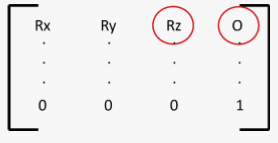
\includegraphics[scale=0.5]{jacobian_elems.png}
\end{figure}

\subsection{ROS Code}

Programmatically, the elements $z_0, z_1, z_2, o_0, o_1, o_3$ mentioned 
in the Calculations subsection above are extracted 
and plugged into the Jacobian framework as seen below from the 
\lstinline{velocity_kinematics.py} file (which is submitted as part of the 
\lstinline{velocity_kin} package).

\lstinputlisting[language=python,firstline=63,lastline=84]{../ros2-code/src/velocity_kin/velocity_kin/velocity_kinematics.py}

At this point, we have the ability to solve for the forward or inverse velocity kinematics. By multiplying the Jacobian by the joint’s velocities matrix, we can solve for the velocity of the end effector. Likewise, if the inverse of the Jacobian is multiplied by the end effector velocity matrix, the velocity of each of the joints can be found. It should be noted that since this particular Jacobian is not square, the inverse cannot simply be taken and therefore the pseudo-inverse numpy function is used in order to take the inverse. Having the Jacobian solved and regularly available allows us to calculate the forward and inverse velocity kinematics and therefore create a controller for the robot so achieve the desired movement and speed.

\section{Velocity Controller}

The process of creating a controller for this application stems from the previous
position controller as well as other controllers created throughout the course.
The goal velocity of each joint, $V_r$ is is received through a service response.
The name of the service is \lstinline{velocity_inv_kin_service}. Suppose our current
velocity is given as $V$.
The error for each joint is then calculated as follows:
\[
    E = V_r - V
\]

When paired with the proportional gain value, we now have one of the terms of the controller. In order to get the other term, the derivative of the error is also needed, and is calculated as shown: 

\[
    \dot{E} = \frac{V - V_{prev}}{\Delta time}
\]

This derivative of the error is paired with the derivate gain and now completes the controller. Our controller takers on the form: 

\[
    F = K_p E + K_d \dot{E}
\]
Where F is the effort that will be applied in Gazebo and will cause the joints to move.

\end{document}